\documentclass[11pt]{article}

% ------------------------------------------------
% 1. Packages
% ------------------------------------------------
\usepackage[utf8]{inputenc}
\usepackage[T1]{fontenc}
\usepackage[margin=1in]{geometry}
\usepackage{xcolor}
\usepackage{amsmath}
\usepackage[most]{tcolorbox}
\usepackage{xr}         % Referans okuma
\usepackage{clipboard}  % Metin okuma
\usepackage{etoolbox}   % Döngü işlemleri
\usepackage{graphicx}
\input{preamble}


% ------------------------------------------------
% 2. Manuscript Connection
% ------------------------------------------------
\externaldocument{latex_output/article} % Sayfa numaralarını al
\externaldocument{latex_output/supplement}
\openclipboard{latex_output/article}    % Metin içeriğini al (.cpy dosyasından)

\usepackage{cleveref}
\crefname{subsection}{Section}{Sections}
\Crefname{subsection}{Section}{Sections}
\crefname{section}{Section}{Sections}
\Crefname{section}{Section}{Sections}
\crefname{hypothesis}{Hypothesis}{Hypotheses}
\crefname{fact}{Fact}{Facts}
\crefname{assumption}{Assumption}{Assumptions}
\crefname{definition}{Definition}{Definitions}
\crefname{proof}{Proof}{Proofs}
\crefname{lemma}{Lemma}{Lemmas}
\crefname{figure}{Figure}{Figures}

% ------------------------------------------------
% 3. Color Palette (SENİN SEÇİMLERİN)
% ------------------------------------------------
% Ana Kutu (ReviewCycle)
\definecolor{boxframe}{RGB}{40, 60, 100}     
\definecolor{boxfill}{RGB}{250, 250, 252}    

% Reviewer (Kiremit/Gri)
\definecolor{revbg}{RGB}{250, 240, 240}      
\definecolor{revtitle}{RGB}{180, 50, 50}     

% Author (Senin istediğin Gri Tonu)
\definecolor{authbg}{RGB}{235, 235, 235}     
\definecolor{authtitle}{RGB}{0, 80, 120}     

% Revision (Alice Blue - Değişmedi)
\definecolor{revisionbg}{RGB}{240, 248, 255} 

% ------------------------------------------------
% 4. Environments & Macros
% ------------------------------------------------

% A. Ana Çerçeve (ReviewCycle)
\newtcolorbox{ReviewCycle}[1]{
    enhanced, breakable, width=\textwidth,
    colframe=boxframe, colback=boxfill,
    coltitle=white, fonttitle=\bfseries\sffamily,
    title={#1}, arc=3pt, boxrule=0.8pt,
    top=5pt, bottom=5pt, left=5pt, right=5pt,
    drop fuzzy shadow,
    before upper={\parskip 0.5em}
}

% B. Reviewer Kutusu
\newcommand{\ReviewerText}[1]{%
    \begin{tcolorbox}[
        enhanced, frame hidden, colback=revbg,
        left=5pt, right=5pt, top=5pt, bottom=5pt, arc=2pt
    ]
        \textbf{\textcolor{revtitle}{Comment:}} 
        \itshape \textcolor{black!80}{#1}
    \end{tcolorbox}
    \vspace{0.05cm}
}

% C. Author Kutusu
\newcommand{\AuthorResponse}[1]{%
    \begin{tcolorbox}[
        enhanced, frame hidden, colback=authbg,
        left=5pt, right=5pt, top=5pt, bottom=5pt, arc=2pt
    ]
        \textbf{\textcolor{authtitle}{Response:}} 
        \normalfont \textcolor{black}{#1}
    \end{tcolorbox}
    \vspace{0.1cm}
}

% D. Akıllı Revizyon Kutusu (Çoklu ID Destekli)
\newcommand{\AutoRevision}[1]{%
    \begin{tcolorbox}[
        enhanced, breakable,
        colback=revisionbg, frame hidden,
        borderline west={3pt}{0pt}{blue!40}, % Mavi çizgi
        left=5pt, right=5pt, top=5pt, bottom=5pt,
        arc=2pt 
    ]
        % Başlık
        \textbf{\textcolor{blue!40!black}{Revisions in Manuscript:}}
        
        % ID Listesi üzerinde döngü (örn: 1.2a, 1.2b)
        \renewcommand{\do}[1]{%
            \par\vspace{0.3cm} % Maddeler arası boşluk
            
            % 1. Konum Bilgisi (Section X, Page Y)
            {\small\bfseries\color{blue!60!black} $\hookrightarrow$ Section \ref{rev:##1}, Page \pageref{rev:##1}:}
            
            % 2. Metin (Alt satıra yapıştır)
            \par\nopagebreak
            \begingroup
            \itshape\small \Paste{text:##1}
            \endgroup
        }
        \docsvlist{#1} % Listeyi işle
    \end{tcolorbox}
}


% E. Plain Revizyon Kutusu 
\newcommand{\PlainRevision}[1]{%
    \begin{tcolorbox}[
        enhanced, breakable,
        colback=revisionbg, frame hidden,
        borderline west={3pt}{0pt}{blue!40}, % Mavi çizgi
        left=5pt, right=5pt, top=5pt, bottom=5pt,
        arc=2pt
    ]
        % Başlık
        \textbf{\textcolor{blue!40!black}{Possible Revisions in Manuscript:}}

        \docsvlist{#1}
        
    \end{tcolorbox}
}

% ------------------------------------------------
% 5. Document Content
% ------------------------------------------------
\begin{document}

\begin{center}
    {\Large \textbf{Response to Reviewers}}\\[0.5em]
    \textbf{Paper:} A Unified Analysis of Generalization and Sample Complexity for Semi-Supervised Domain Adaptation
\end{center}
\hrule \vspace{1em}

\begin{ReviewCycle}{Reviewer 1, Comment 1}
    \ReviewerText{Below Theorem 1, there is a claim that “This statement holds with probability approaching 1 at an exponential rate with the increase in number of labeled samples $M_s$”, which seems to be unrigorous. Since the second term w.r.t. the target domain in Eq. (5) would not vanish unless $\alpha=0$, the term seems to serve as a constant. Detailed justifications are expected.
    }
    \AuthorResponse{No action needed.}
    % \AutoRevision{1.1}
\end{ReviewCycle}


\begin{ReviewCycle}{Reviewer 1, Comment 2}
    \ReviewerText{
        The setting of the kernel map in Section 3.2 looks strange. Specifically, if the mappings $f^s$ and $f^t$ for the shared representation learning are both set as $\phi$, how could $\phi$ ensure that the original spaces $\mathcal{X}^s$ and $\mathcal{X}^t$ are projected into the same space? Moreover, in such a setting, this theory may be limited to the scenarios that the source space and target space share the same or similar structures, e.g., it would fail in the heterogeneous cases.
    }
    \AuthorResponse{Reviewer Section 3.2 demiş ama sanırım 2.3'ü kastediyor. Kafa karışıklığını önlemek için Section 2.3'teki kernel map discussion'u, Remark 2 ile birleştirilerek footnote olarak yazıldı. Bu sayede $\fs = \ft$ varsayımının $\Xs = \Xt$ varsayımından geldiği; ama bizim böyle bir varsayımı yine de kullanmadığımız açıkça ifade edilmiş oldu. Bonus olarak yer kazanmış olduk.
    }
    \AutoRevision{1.2}
    % \PlainRevision{
        
    % \begin{equation}
    %     dfdsfg = 3x^2
    % \end{equation}
    
    % \begin{itemize}
    %     \item dfdsfg = 3x^2
    %     \item dfdsfg = 3x^2
    % \end{itemize}

    % }
\end{ReviewCycle}


\begin{ReviewCycle}{Reviewer 1, Comment 3}
    \ReviewerText{
        The finite variance/moment assumption, i.e., Assumption 3, needs further clarification. In the current version, there is a simple justification that “these assumptions hold for many common data distributions in practice”. Since this assumption is important, it would be helpful to provide a more informative discussion, e.g., which types of data would satisfy this condition, or what conditions are necessary for the data?
    }
    \AuthorResponse{Hocam yanlış anlamadıysam bounded input ve neural networkler için bu varsayım direkt geçerli. Bunları da zaten Assumption 5'te ve Lemma 7'de gösteriyoruz. Aşağıdaki açıklamaları da "These assumptions hold for many common data distributions in practice" cümlesine bir footnote olarak ekledim:}
    \AutoRevision{1.3}
\end{ReviewCycle}

\begin{ReviewCycle}{Reviewer 1, Comment 4}
    \ReviewerText{
        Following the last question, if the functions $f^s$ and $f^t$ are related to the RKHSs, it would also be helpful to clarify the connection between the assumption and the kernels. Specifically, the finite assumption on kernel-based statistics would be closely related to the choices of kernels.
    }
    \AuthorResponse{Belki Comment 1.3 bu doğrultuda improve edilebilir fakat ben bu comment'e özel bir aksiyon almadım.}
    %\AutoRevision{}
\end{ReviewCycle}


\begin{ReviewCycle}{Reviewer 1, Comment 5}
    \ReviewerText{
        The convergence bound of empirical MMD seems to have already been studied in existing literature. It would be helpful to discuss the differences between the results in Lemma 3 and existing bounds.
    }
    \AuthorResponse{Hocam sanırım Gretton et al. (2012) A Kernel Two-Sample Test makalesinde bazı boundlar var. Üzerinde detaylı düşünemedim ve makalede bu konuyla ilgili bir değişiklik yapmadım fakat bilginize sunarım (ekran alıntısı adı geçen makaleden):}
    \begin{center}
      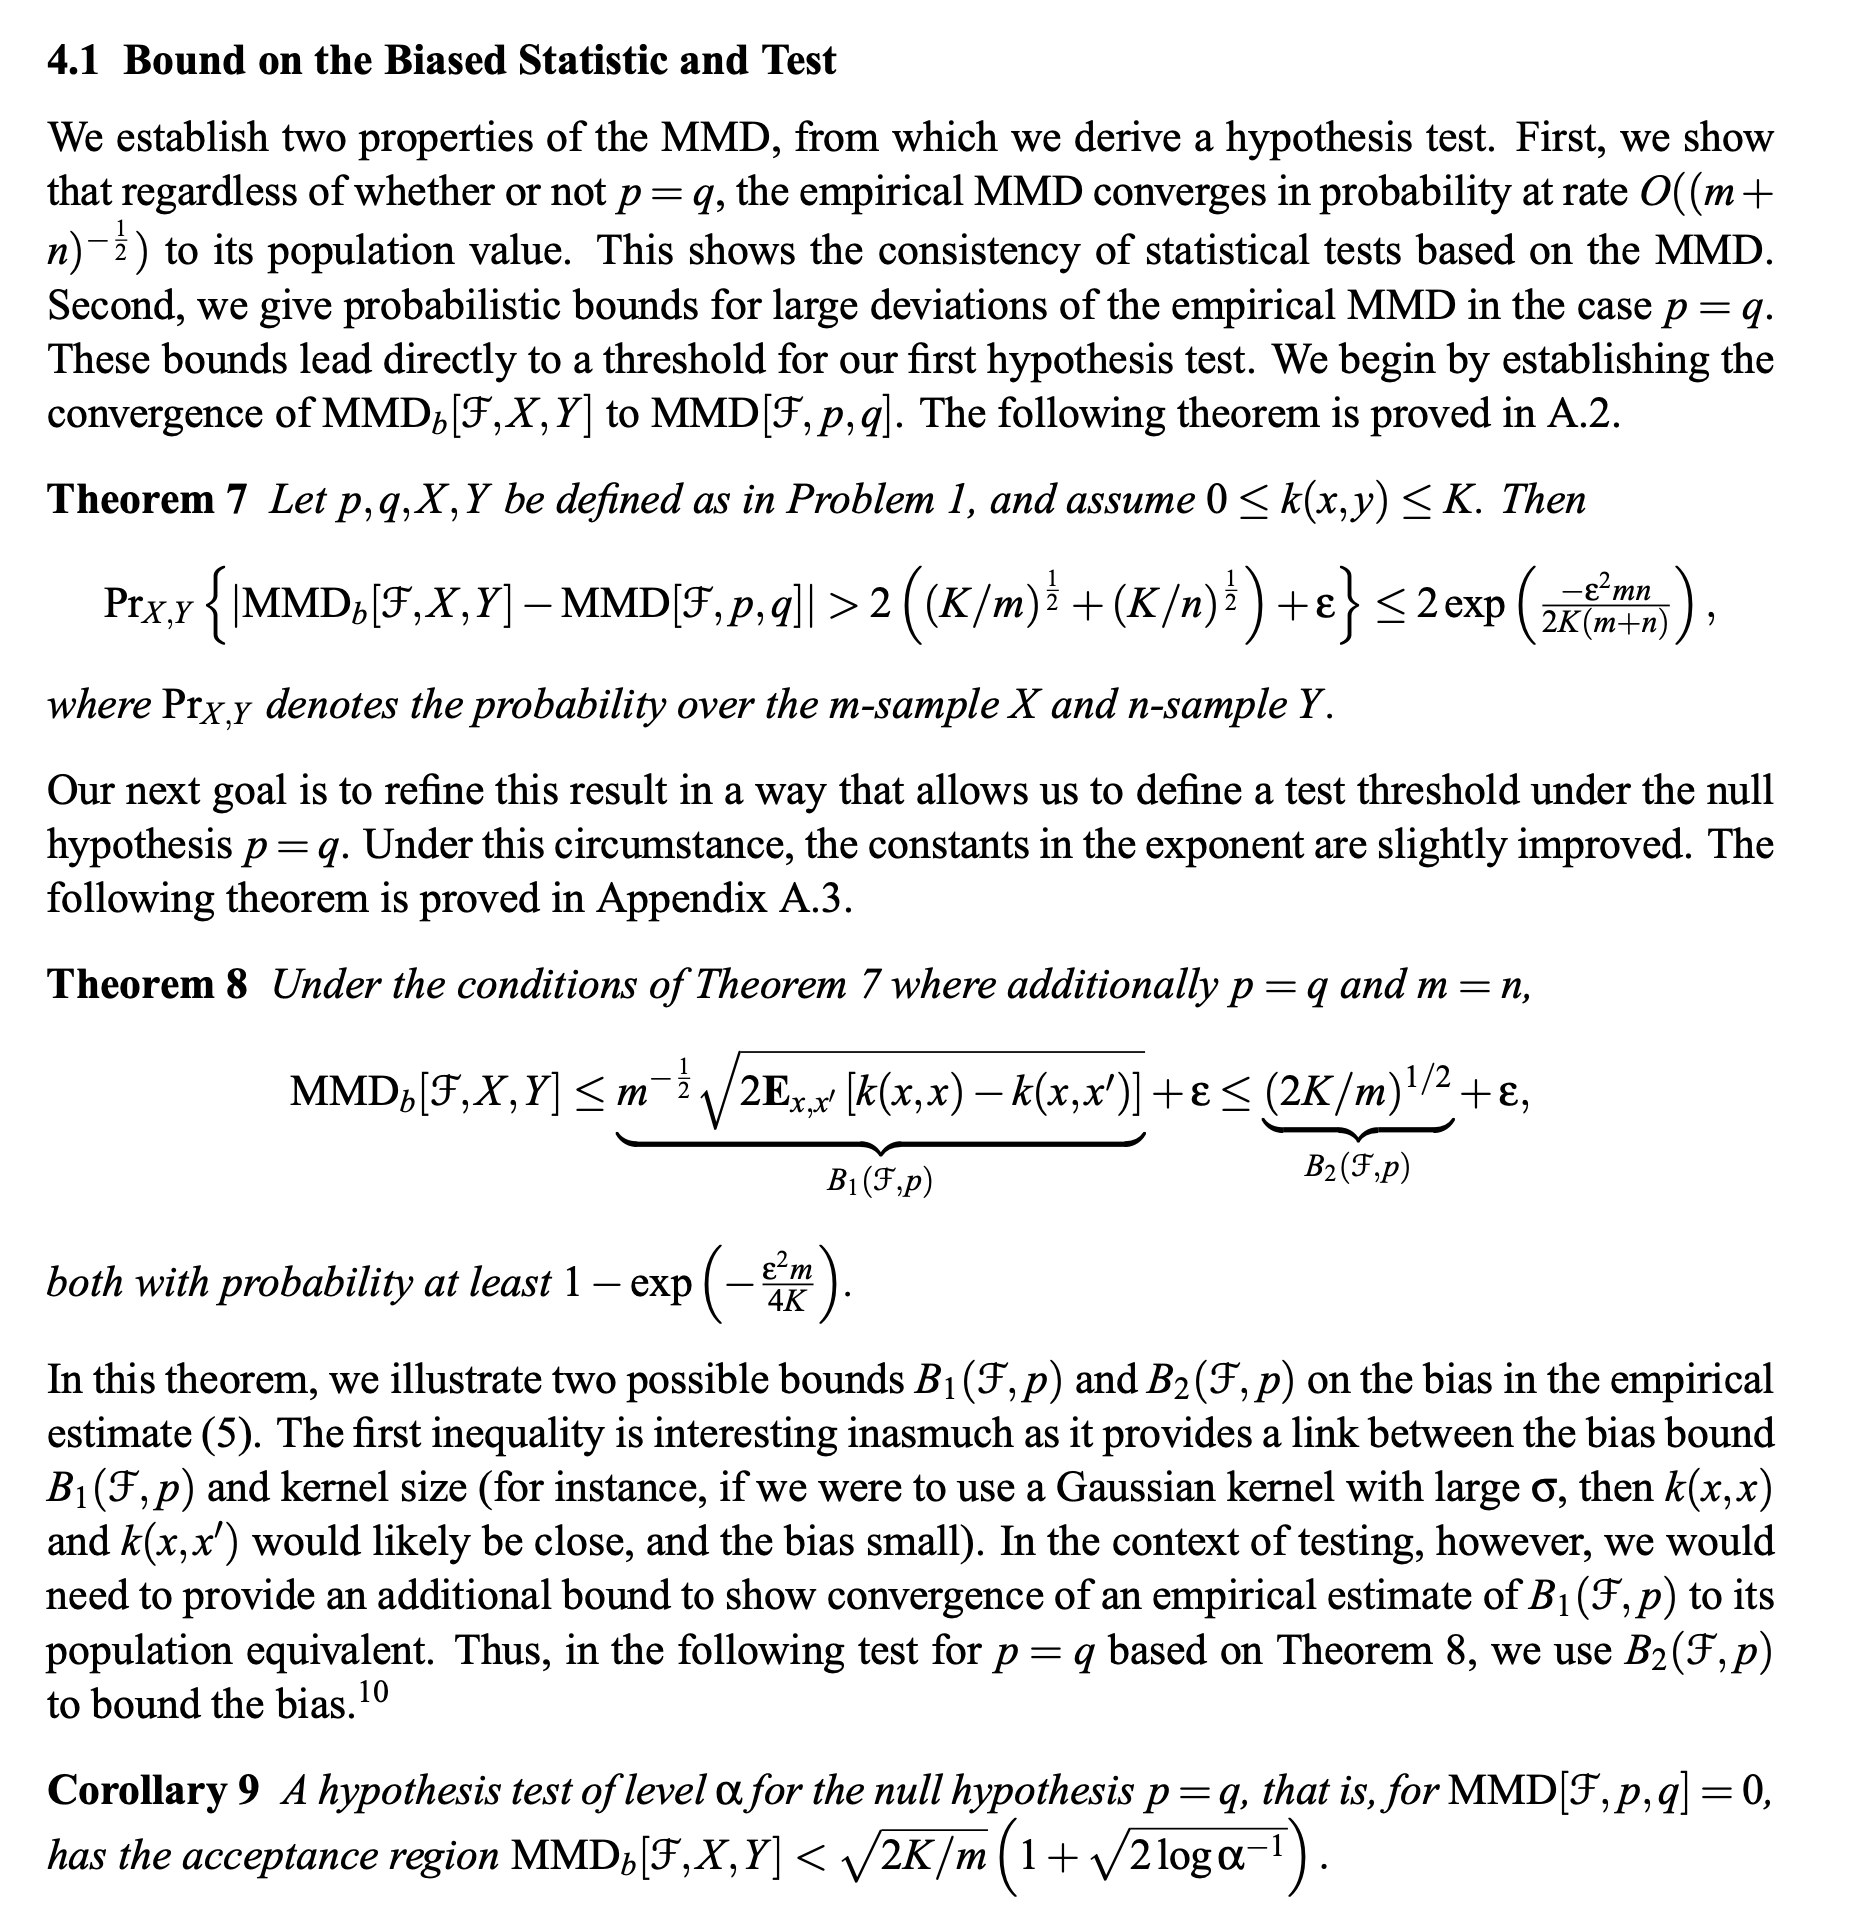
\includegraphics[width=0.5\textwidth]{gretton-thm7-8.png}
    \end{center}
    %\AutoRevision{}
\end{ReviewCycle}


\begin{ReviewCycle}{Reviewer 1, Comment 6-7}
    \ReviewerText{
        As far as I understand this submission, the major results are the generalization bound in Theorem 1 and its connection to specific algorithms that characterize the discrepancy $D(f^s,f^t)$. However, an important prior is Assumption 1, which can be taken as a stronger version of the change of measure inequality. Note that the L.H.S. of Eq. (3) is dominated by both variables $X$ and $Y$, while the R.H.S. (i.e., $D(f^s,f^t)$) seems to only depend on $X$. Such scenarios make this assumption less informative or too strict. More discussion would be helpful.
    }
    \ReviewerText{
        Following the last question, the analysis on sample complexity under popular learning algorithms is interesting, but the constant $R$ is also important, in my understanding. It seems that the constant $R$ is unjustified throughout this manuscript. It would be expected to show the nature of $R$ explicitly, e.g., how MMD-based network and domain adversarial network satisfy Assumption 1 and what are their corresponding values of $R$.
    }
    \AuthorResponse{Bu konuya eğileceğiz (Assumption 1).}
    % \AutoRevision{1.6a, 1.6b}
\end{ReviewCycle}

\begin{ReviewCycle}{Reviewer 1, Comment 8}
    \ReviewerText{
        The result $\alpha_{optimal}=O(\sqrt{M_t})$ is consistent with the empirical observation, which is good. However, since $\alpha$ should be set within $(0,1)$, is there any further suggestion for a practical setting for it?
    }
    \AuthorResponse{No action needed.}
    %\AutoRevision{}
\end{ReviewCycle}
\begin{ReviewCycle}{Reviewer 2, Comment 1}
    \ReviewerText{
        The paper relies on assumptions that may not hold in practical domain adaptation scenarios. For example, The theoretical framework relies on Assumption 1, which posits a linear bound between the loss difference and distribution discrepancy (e.g., |Ls - Lt|<=RD(fs,ft)). This assumption may not hold in complex real-world scenarios where domain shifts involve non-linear or high-dimensional disparities, such as label skew or heterogeneous data structures. For instance, the paper acknowledges that domain adaptation must handle "covariate shift, label shift, and heterogeneous settings", yet the assumption simplifies these into a uniform bound. Strengthening this by incorporating more flexible discrepancy measures (e.g., conditional distributions) could improve robustness.
    }
    \AuthorResponse{Bu konuya eğileceğiz (Assumption 1).}
    % \AutoRevision{2.1}
\end{ReviewCycle}

\begin{ReviewCycle}{Reviewer 2, Comment 2}
    \ReviewerText{
        The sample complexity bounds derived for neural networks (e.g., quadratic scaling with width and depth) are not proven to be tight. The paper acknowledges that these bounds are pessimistic but does not compare them to empirical scaling or provide lower bounds, limiting their practical utility. For example, the sample complexity bounds depend heavily on covering numbers of function classes. However, for deep neural networks, covering numbers are often computationally intractable to estimate and can lead to loose bounds that scale quadratically with depth/width ($O(d^2 L^2)$).
    }
    \AuthorResponse{No action needed.}
    % \AuthorResponse{Hocam sanki bu yorum ve hakemin diğer yorumları, neural networklerle ilgili herhangi bir teori yapılamaz varsayımından ileri geliyor gibi. Resmen covering numbers neural network'ler için tractable değildir ve loose bound'lara lead eder diyip geçilmiş. Biraz ciddiye almaya değmez gibi geldi. Ayrıca sonuç olarak gerçek hayatta çalıştığını gösteren deneylerimiz var, onların anlamı nedir öyleyse? Deneylerimizde kullanılan networklerin gerçek hayatta kullanılan networklerden farklı olduğunu düşünmüş olabilir (drop out vs şeyler kullanılmadığı için). Burada biraz haklı olur. Aslında overfitting rejimine girmesi için sadece data ile oynadığımızı hatırlıyorum, eğer orijinal kodlarda kullanılan bir overfitting mitigation stratejisi varsa, ben onları kasten kaldırmadım. Belki deneylerimizin gerçek hayatta kullanılan neural network traininglerine çok benzediği gibi bir savunma yapabiliriz, eğer geçerli bir savunma olursa bu. Başka bir comment'te de (comment 2.4) bundan bahsedilmişti. Hüseyin, sen yine de şunları düşün:
    % 1- Burada covering numbers'a bağlı bir sample complexity hesabı olduğunu söylemiş, ama biz makalemizde bunu kullanmıyoruz. 
    % 2- Intractability problemimiz bizim de var mı? }
    %\AutoRevision{}
\end{ReviewCycle}

\begin{ReviewCycle}{Reviewer 2, Comment 3}
    \ReviewerText{
        Assumption 5 restricts network parameters to a bounded set. While this simplifies analysis, it contradicts common practices where parameters are regularized but not strictly bounded. In real training, unbounded optimization (e.g., via gradient descent) could violate this assumption, undermining the generality of the bounds. Incorporating norm-based regularization explicitly into the theory would align better with empirical practices.
    }
    \AuthorResponse{No action needed.}

    %\AutoRevision{}
\end{ReviewCycle}

\begin{ReviewCycle}{Reviewer 2, Comment 4}
    \ReviewerText{
        The experiments deliberately maintain networks in the overfitting regime to study sample complexity. While this isolates the effect of network size, it ignores practical techniques like dropout or early stopping that mitigate overfitting. Consequently, the reported sample complexities (e.g., $O(d^2 L^2)$) may be overstated for real-world applications. Including ablation studies with regularization could provide a balanced view.
    }
    \AuthorResponse{Hocam ana metinden "deliberately kept in overfitting regime" ifadesini kaldırdım, ve deneylerle ilgili detay verdiğimiz footnote'lara aşağıdaki ifadeleri açıkça ekledim. Bunları daha da öne çıkarıp, bir remark olarak mesela, ifade etmek de mümkün tabii. Yani teorik analizimizde dahil etmedik ama deneysel olarak gösterdik ki bulgularımız gerçek hayat pratikleriyle tutarlı gibisinden.}
    \AutoRevision{2.4a, 2.4b}
\end{ReviewCycle}

\begin{ReviewCycle}{Reviewer 2, Comment 5}
    \ReviewerText{
        The experiments focus on specific architectures (e.g., MMD-based networks and adversarial networks). The paper notes that "convolutional layers are left out of the scope" in some analyses, which reduces relevance to modern architectures like Transformers or ResNets. Testing a broader range of models would strengthen the claims about generalizability.
    }
    \AuthorResponse{Bu doğrultuda aşağıdaki footnote eklendi:}
    \AutoRevision{2.5}
\end{ReviewCycle}

\end{document}